%%%%%%%%%%%%%%%%%%%%%%%%%%%%%%%%%%%%%%%%%%%%%%%%%%%%%%%%%%%%%%%%%%%%%%%%%%%%%%%%
\pagebreak
\section{Introduction}

%%%%%%%%%%%%%%%%%%%%%%%%%%%%%%%%%%%%%%%%%%%%%%%%%%
\subsection{Motivation}
\todo{why is grasping important}

%%%%%%%%%%%%%%%%%%%%%%%%%%%%%%%%%%%%%%%%%%%%%%%%%%
\subsection{Use Case}
\todo{describe Robocup use case}

%%%%%%%%%%%%%%%%%%%%%%%%%%%%%%%%%%%%%%%%%%%%%%%%%%
\subsection{An overview of robotic grasping research}

Synthesizing an optimal grasp from perceptual data is a challenging problem and is frequently addressed in
robotic research, resulting a myriad of approaches. Sahbani et al. \cite{Sahbani2012} classify grasp synthesis
into analytical and empirical approaches. Analytical methods consider mechanical properties of the contact
points between the gripper's fingers and an object \cite{Roa2015,Sahbani2012,Shimoga1996}, namely:
\begin{itemize}
\item Disturbance resistance: ability of the grasp to resist disturbances when the object is immobile, either by
form-closure (finger positions) or force-closure (forces applied by fingers).
\item Dexterity: ability of the robot hand to move the object to perform a specified task, or in any direction if
no task is specified.
\item Equilibrium: the combined forces and torques applied onto the object is null.
\item Stability: any displacement of an object caused by a disturbance will self-correct over time.
\end{itemize}
Instead of analyzing mechanical properties, empirical approaches rely on some form of grasp experience to synthesize
candidates. Sahbani et al. \cite{Sahbani2012} group empirical approaches based on whether they focus on observing humans
or objects. The first group of methods teach a robotic system to observe a human operator via different forms of
descriptors, then to reproduce the same grasp. These techniques are also known as learning by demonstration.
Methods focusing on object observation in general learn the association between object characteristics and gripper
configurations. The survey by Bohg et al. \cite{Bohg2014} argues instead to classify data-driven methods based on how
much information is assumed about the query object, specifically:
\begin{itemize}
    \item Approaches dealing with \emph{known objects} rely on a grasp experience database which contain suitable grasps
    for each encountered object. These approaches, therefore, focus on object recognition and pose estimation.
    \item Approaches for \emph{familiar objects} focus on finding a similarity metric and an object representation,
    from low (i.e. shape, color, texture) to high (i.e. category) levels, to match query objects with encountered
    objects.
    \item Approaches for \emph{unknown objects} identify local or global features from sensory data to for generating
    and evaluating grasp candidates.
\end{itemize}
The authors argue that this classification can better capture the diversity of empirical approaches as well as
the importance of perception in the process. In addition to the above classification, Bohg et al. \cite{Bohg2014}
also identify principal factors that may influence a grasp hypothesis, as shown in the mind map in figure
\ref{fig:grasp_synthesis_mind_map}.

\begin{figure}[H]
    \centering
    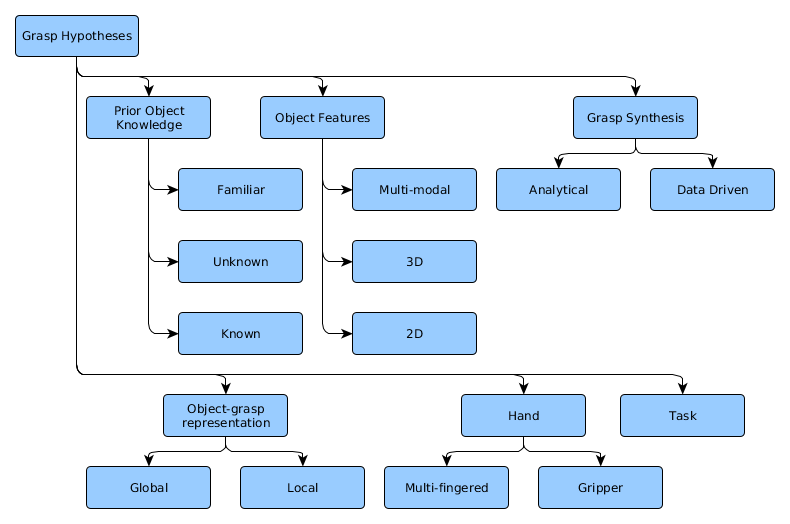
\includegraphics[width=0.9\textwidth]{bohg14-grasp_synthesis_mind_map}
    \caption{Aspects which may influence generation of grasp hypotheses \cite{Bohg2014}.}
    \label{fig:grasp_synthesis_mind_map}
\end{figure}

Analytical approaches to synthesizing grasps generally rely on knowledge of the object, the gripper model and the
contact location of the fingers. These information is often inaccurate or unavailable in the real environment
because of noisy sensors as well as imprecise manipulator/gripper actuation. Indeed, analytical methods have been
shown to be unreliable in synthesizing stable grasps when applied on real robots
\cite{Kappler2015, Rubert2017, WeiszAllen2012}. Empirical approaches, however, as with other supervised machine
learning methods, demand data. Generating a sufficiently large grasp experience knowledge base is often time-consuming
and expensive, while grasp simulation may not be close enough to the real world.

Data augmentation, the process of generating new samples by transforming real data, and data synthesis are popular
solutions to supplementing limited training data \cite{Fawzi2016, Shrivastava2017}, especially when applying deep
learning methods to solve image recognition and detection tasks. As grasp synthesis algorithms need 3D information
synthesizing the gripper configuration, RGB-D is often preferred over images as training data. The research in
\cite{Eitel2015,Gupta2014RGBDFeatures} proposes approaches to augmenting RGB-D data, whereas Mahler et al.
\cite{mahler2017} generates synthetic data to train a grasp quality predictor.

\todo{narrow to empirical techniques using labeled data}

\todo{layout of the report}
%%%%%%%%%%%%%%%%%%%%%%%%%%%%%%%%%%%%%%%%%%%%%%%%%%%%%%%%%%%%%%%%%%%%%%%%%%%%%%%%
\pagebreak
\section{Related Work}
Empirical grasp synthesis techniques based on labeled data vary mainly in what type of perceptual data is taken into
consideration, how object-grasp representation is formulated based on such perceptual data, and how grasps are
evaluated. This section will review these aspects are handled in recent methods, as well as approaches to augment and
synthesize data relevant to grasping.

%%%%%%%%%%%%%%%%%%%%%%%%%%%%%%%%%%%%%%%%%%%%%%%%%%
\subsection{Extracting features from perceptual data for grasping}
\begin{figure}
    \centering
    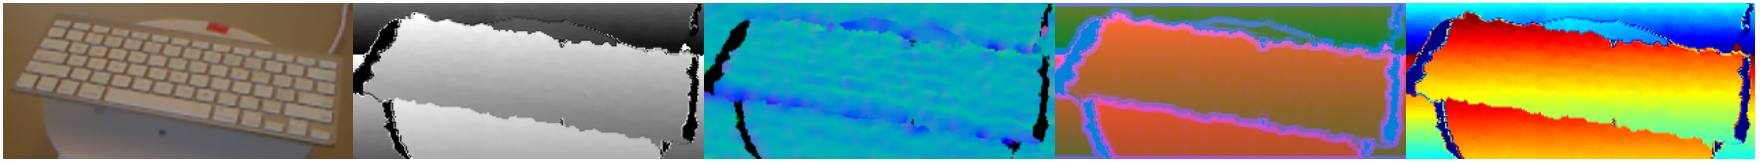
\includegraphics[width=\linewidth]{Eitel_et_al-2015-depth_color_encodings}
    \caption{Different encodings of depth information \cite{Eitel2015}. From left: RGB, grayscale depth, surface normals
        \cite{Bo2013}, HHA \cite{Gupta2014RGBDFeatures}, and the color mapping of depth values proposed by Eitel et al.
        \cite{Eitel2015}.}
    \label{fig:depth-encodings}
\end{figure}

As RGB-D cameras become more accessible and affordable, they are often chosen in robotic systems as the primary
perception sensor. While RGB-D data has been shown to provide richer features compared to pure 2D images for various
perception tasks \cite{lenz2015,Eitel2015,Gupta2014RGBDFeatures,jiang2011}, it is often unclear how to handle the
multi-modality of color and depth information.

Lenz et al. \cite{lenz2015} used deep auto-encoders to build a representation for each feature channel, reducing its data
dimensions. To handle the multi-modality of RGB and depth data, the authors also introduced a structured regularization
technique. Each modality (i.e. RGB and depth/surface normal) has a regularization term which will be added to each
hidden unit. In case of a $p-norm$, with $K$ hidden units, $R$ modalities, and N visible units, the regularization term
would be
\[f(W) = \sum\limits^K_{j=1} \sum\limits^R_{r=1} \left( \sum\limits^N_{i=1} S_{r,i} \lvert W^p_{i,j} \rvert \right)
^{1/p}, \]
where $S_{r,i}$ is $1$ if feature $i$ belongs to modality $r$ and $0$ otherwise.

Bo et al. \cite{Bo2013} built sparse coding dictionaries for RGB-D data using the K-SVD algorithm, and proposed to use
hierarchical matching pursuit (HMP) to compute a feature hierarchy for new RGB-D images. Each entry in the dictionaries
contain 8 channels calculated from RGB-D data: grayscale intensity, RGB, depth and surface normals in three axes.

In order to leverage the success of Convolutional Neural Networks (CNN) in capturing 2D features \cite{Gu2018}, several
multi-modal approaches convert depth data into three-channel images during the preprocessing step
\cite{Eitel2015,Gupta2014RGBDFeatures}. Gupta et al. \cite{Gupta2014RGBDFeatures} proposes the HHA representation, which
encode the depth each pixel of the depth image with horizontal disparity, height above ground, and the angle between the
local surface normal and direction of gravity. Eitel et al. \cite{Eitel2015} proposes to use convert the depth value
directly into RGB values using a jet color mapping. Examples of the different depth encodings can be seen in figure
\ref{fig:depth-encodings}. Two CNN models of the same architecture are then trained independently using depth and RGB
images to classify objects. Finally, features learned from the two models (the networks up until before the
classification layer) are concatenated as inputs to a fully connected layer which learns to combine them to recognize
objects. The paper showed that while surface normals proved to give better classification performance using depth
information alone, they require additional calculation on the input data and does not improve on results when combining
both RGB and depth images compared to the proposed color map encoding.

%%%%%%%%%%%%%%%%%%%%%%%%%%%%%%%%%%%%%%%%%%%%%%%%%%
\subsection{Object-Grasp representation}
Bohg et al. \cite{Bohg2014} parameterized grasps by (1) the \emph{grasping point} of the object where the gripper
should be aligned, (2) an \emph{approach vector} from which the gripper shall approach the \emph{grasping point},
(3) the \emph{wrist orientation} of the robotic hand, and (4) an \emph{initial gripper configuration}.
The article also categorized object-grasp representation approaches into ones which extract local (i.e. curvature,
contact area with the hand) or global features (center of mass, bounding box).

%%%%%%%%%%%%%%%%%%%%%%%%%%%%%%
\subsubsection*{Techniques based on global features}
As illustrated in figure \ref{fig:dexnet-data-gen}, Mahler et al. represent grasps in 2D images by aligning the image
center to the gripper central point and the image's middle row to the grasp axis \cite{mahler2017}. The grasp is assumed
to have an approach vector perpendicular to the table, and hence is characterized by the gripper center and the angle of
the gripper axis with respect to the table.
\begin{figure}[H]
    \centering
    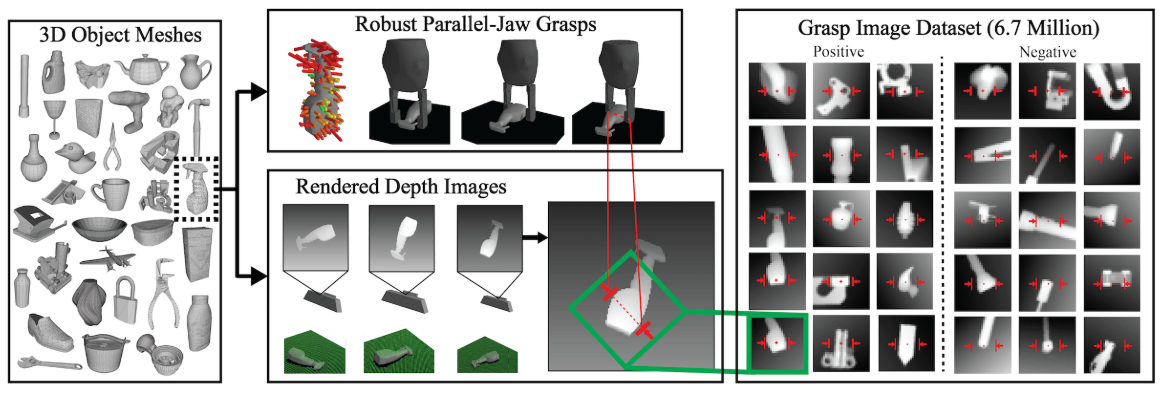
\includegraphics[width=\linewidth]{mahler_et_al-2017-dexnet_2-dataset_generation.png}
    \caption{Dex-net 2.0 data generation pipeline \cite{mahler2017}.}
    \label{fig:dexnet-data-gen}
\end{figure}

Several methods use eigengrasps to represent the object-grasp relation in free space \cite{Goldfeder2011,Ciocarlie2009}.
Ciocarlie and Allen \cite{Ciocarlie2009} introduced eigengrasps and defined them as principal components of the dataset
of human hand configurations. Using this low-dimensional representation, the robot hand receive adjustments from a human
operator during grasp execution. The proposed Eigengrasp planner uses a simulated annealing algorithm to maximize a
quality metric $Q$ calculated from robot hand's posture and pose, where posture is represented using an eigengrasp.
Specifically,
\[ Q = \Sigma_i (1 - \delta_i) \]
for all desired contacts $i$, where
\[
\delta_i = \cfrac{|\mathbf{o_i}|}{\alpha}
+ \left(1 - \cfrac{\mathbf{\hat{n}_i} \cdot \mathbf{o_i}}{|\mathbf{o_i}|} \right)
\]
, in which the local surface normal $\mathbf{\hat{n}_i}$ and the distance between desired contact location and the
object $\mathbf{o_i}$ is related to the eigengrasp and hand position. $\alpha$ is a scaling factor make the first term
comparable to the second in the latter equation. Goldfeder and Allen \cite{Goldfeder2011} used the Eigengrasp planner
to generate the Columbia Grasp Database. Grasp planning is then done by matching the query object to one in the
database, then executing the best indexed grasp for the matched object.


%%%%%%%%%%%%%%%%%%%%%%%%%%%%%%
\subsubsection*{Techniques based on local features} \label{subsub:object_grasp_local}

Several methods represent grasp candidates as rectangles positioned in RGB and/or depth images \cite{lenz2015,jiang2011},
corresponding with a bipedal gripper. The RGB-D image region within these rectangles is then used to score the
respective grasp using machine learning methods.

Kappler et al. \cite{Kappler2015} extracts local shape representations (or templates) of objects from point clouds
generated from object meshes at various camera view points. The templates are grids with predefined resolution
aligned with the plane tangent to the object surface at intersection point between grasp approach vector and the
object. Each point cloud will be projected onto the grid, where the grid cells with corresponding projected points
``contain the distance to that point as a value,'' and the other grid cells are considered either occlusion
(with height depends on the camera angle) or free space (with fixed height). Figure \ref{fig:local_shape_viewpoints}
illustrates how the local shape representations capture the different camera viewpoints.

\begin{figure}[H]
    \centering
    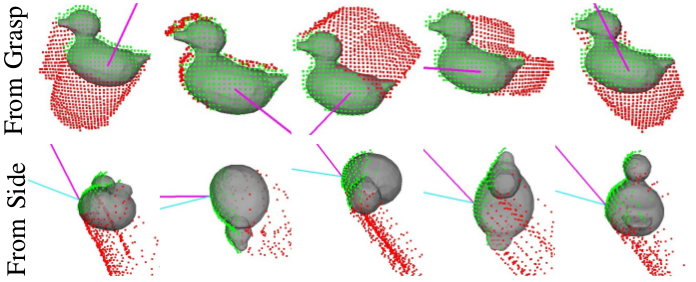
\includegraphics[width=0.8\textwidth]{kappler_et_al-2015-fig8-local_shape_diff_viewpoints.png}
    \caption{Local shape representations with different camera view points of the same grasp. Cyan lines
        represents the approach vectors while pink lines represent the camera viewpoint \cite{Kappler2015}.}
    \label{fig:local_shape_viewpoints}
\end{figure}

Detry et al. \cite{Detry2012} \todo{fill approach}

%%%%%%%%%%%%%%%%%%%%%%%%%%%%%%%%%%%%%%%%%%%%%%%%%%
\subsection{Grasp evaluation}

%%%%%%%%%%%%%%%%%%%%%%%%%%%%%%
\subsubsection*{Quick overview of classical grasp metrics}
\begin{table}[H]
    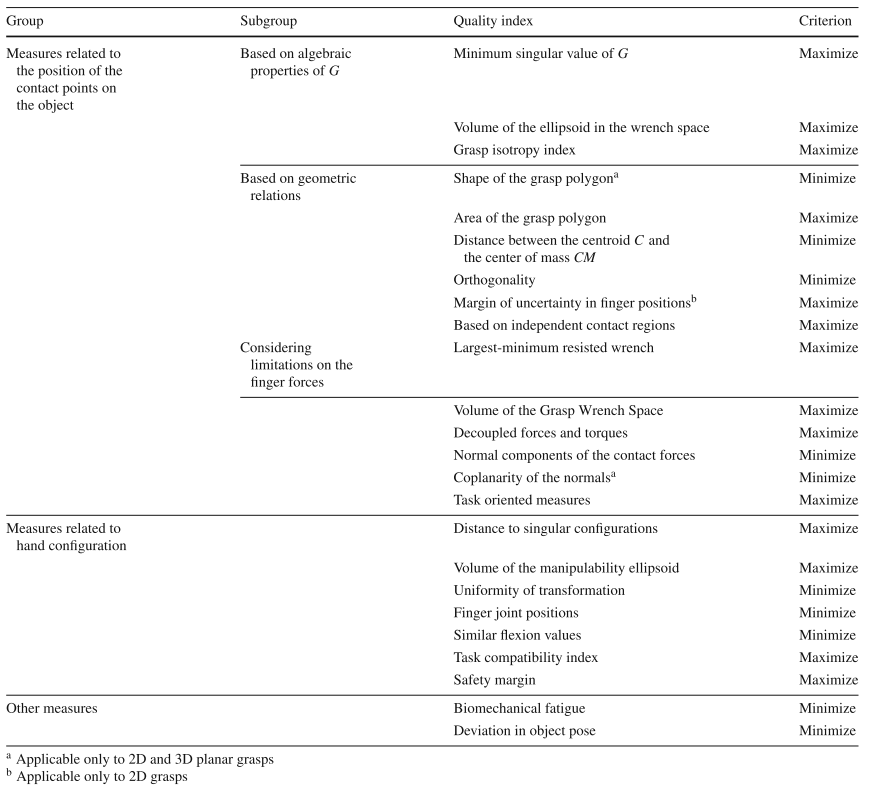
\includegraphics[width=\textwidth]{roa_suarez-2015-grasp_metrics}
    \caption{Grasp quality measures \cite{Roa2015}.}
    \label{table:grasp_metric}
\end{table}

Roa and Su{\'a}rez group grasp quality measures into approaches focusing on contact point position, hand configuration, and ones which combine both metric types \cite{Roa2015}.
\begin{itemize}
    \item Contact point grasp quality measures focus on the object's properties, friction constraints and form/force closure conditions.
    \item Hand configuration measures focus on studying the properties of the hand-object Jacobian $H$.
    \item Grasp measures can be combined serially or in parallel to capture different aspects of a grasp's quality. In the serial approach, one quality measure is applied to find several grasp candidates, then another metric is used to choose the optimal candidate. The parallel approach combines the different measures in a single global index.
\end{itemize}
Table \ref{table:grasp_metric} illustrates how contact point and hand configuration related approaches can be further categorized into subgroups, and include metrics based on bio-mechanical fatigue and deviation of object pose which are not encapsulated by the aforementioned groups.

\todo{$\epsilon$-metric}

%%%%%%%%%%%%%%%%%%%%%%%%%%%%%%
\subsubsection*{Learning to predict grasp quality}
Learning rectangles \cite{mahler2017,jiang2011,lenz2015}
Kappler et al. \cite{Kappler2015}

\todo{to be filled}

%%%%%%%%%%%%%%%%%%%%%%%%%%%%%%%%%%%%%%%%%%%%%%%%%%
\subsection{Generating data for grasp success prediction}

%%%%%%%%%%%%%%%%%%%%%%%%%%%%%%
\subsubsection{Data synthesis}
Several grasp synthesis approaches generate RGB-D images from object meshes at different viewpoints
\cite{mahler2017,Gupta2014RGBDFeatures,Kappler2015} for constructing a grasp knowledge database. These approaches
usually differ in how to \todo{to be filled}

Dex-net \todo{reorganize with other approaches}
\begin{itemize}
    \item Compute stable object poses from 3D mesh models from Dex-Net 1.0 \cite{mahler2016}, object meshes are rescaled
    to fit within the gripper physical constraints, and store poses with probability of occurrence above a threshold.
    \item Grasps are sampled using rejection sampling to ensure coverage of the object surface, ranked and selected
    using a grasp quality metric.
    \item 2D images are generated from grasp candidates as training data with the antipodal axis aligned to the middle
    row of the image.
\end{itemize}

Kappler et al. \cite{Kappler2015}

%%%%%%%%%%%%%%%%%%%%%%%%%%%%%%
\subsubsection{Data augmentation}
Eitel et al \cite{Eitel2015}

\cite{Gupta2014RGBDFeatures}


%%%%%%%%%%%%%%%%%%%%%%%%%%%%%%%%%%%%%%%%%%%%%%%%%%
%\subsection{Task Compatibility}
%    In addition to stability, a successful grasping strategy also has to take into account the task to be performed with the grasped object. However, Sahbani et al. \cite{Sahbani2012} points out that incorporating task compatibility in to grasp synthesis, is still an open challenge because of the difficulty in modeling a task and the computational cost of finding a suitable grasp once a task is defined. These challenges are particularly relevant to analytic grasp synthesis, but is also not solved by empirical approaches. Methods which mimic human grasping alleviate the need for modeling tasks but is not fully automatic when facing new objects, while methods based on object observations have to generate many grasp candidates and face the same difficulty of task modeling as analytical approaches. One possible approach suggested by the article is to directly identify object features that are relevant to the requested tasks. Approaches to task modeling include methods based on manipulability ellipsoids \cite{Yoshikawa1990} and task space polytopes \cite{lee1997}, or building a task compatibility index measuring the similarity between the optimal directions of the manipulator and the movements required by a specific task \cite{chiu1988}.
